%-------------------------------------------------------------------------------

\documentclass{uofsthesis-cs}

\usepackage[pdftex]{graphicx}

%-------------------------------------------------------------------------------

% THESIS TITLE
\title{Play Experience Enhancement Using Emotional Feedback}

% AUTHOR'S NAME
\author{Faham Negini}

% DEGREE SOUGHT
\degree{\MSc}         

% EXPECTED CONVOCATION DATE
\convocationdate{September/2013}

% NAME OF ACADEMIC UNIT
\department{Computer Science}
% \academicunit{Division}

% PERMISSION TO USE ADDRESS
\ptuaddress{Head of the Department of Computer Science\\
176 Thorvaldson Building\\
110 Science Place\\
University of Saskatchewan\\
Saskatoon, Saskatchewan\\
Canada\\
S7N 5C9
}

%-------------------------------------------------------------------------------

\abstract          {% Abstract less than or equal to 1 page
% one page stating what the thesis is about
% highlight the contributions of the thesis

Innovations in computer game interfaces continue to enhance the experience of players. Affective games –those that adapt or incorporate a player’s emotional state – have shown promise in creating exciting and engaging user experiences. However, a dearth of systematic exploration into what types of game elements should adapt to affective state leaves game designers with little guidance on how to incorporate affect into their games. We created an affective game engine, using it to deploy a design probe into how adapting the player’s abilities, the enemy’s abilities, or variables in the environment affects player performance and experience. Our results suggest that affectively adapting games can increase player arousal. Furthermore, we suggest that reducing challenge by adapting non-player characters is a worse design choice than giving players the tools that they need (through enhancing player abilities or a supportive environment) to master greater challenges.}
\acknowledgements  {First and foremost thanks God for bestowing me the ability to learn, to speak and to write. For all of the oppurtinities and all of His mercy and compassion I have experienced throughout my life.\\

I would like to express my sincere gratitude to my advisors Prof. Regan Mandryk  and Prof. Kevin G. Stanley for the continuous support of my M.S. study and research, for their patience, motivation and friendliness. Their guidance helped me in all the time of research and writing of this thesis. I could not imagine having any better advisors and mentors for my M.S. study.\\

Besides my advisors, I would like to thank the rest of my thesis committee: Prof. , Prof. , and Dr. , for their encouragement, insightful comments, and hard questions.\\

My sincere thanks also goes to Dr. Daniel Neilson, Gwen Lancaster, Shakiba Jalal and Dr. Stanley for offering me the internship opportunities and leading me working on diverse exciting projects.\\

I would like to thank my wife Farzane Jenaban for her pacience, understanding and support in every single moment my attention was away from her towards this research and thesis; And my parents Mohammad Negini and Farzaneh Sarmadi, for their spiritual support throughout my life.\\

Last but not the least I thank my fellow labmates in DISCUS and HCI Labs: Mohammad Hashemian, Amin Tavassolian, Ariyan Zohoorian, Farjana Eishita, Max Birk, Michael Kalyn, Michael Bullock and Steve Sutcliffe, for the stimulating discussions, for the nights we were working together, and for all the fun we have had in the last years. Also I thank all of my other friends in University of Saskatchewan.\\
}
%\dedication       {This is the thesis dedication (optional)}
\loa               {\abbrev{TT}   {Thought Technology}
\abbrev{GSR}  {Galvanic Skin Response}
\abbrev{EMG}  {Electromyography}
\abbrev{EKG}  {Electrocardiography}
\abbrev{ECG}  {Electrocardiography}
\abbrev{HF}   {High-frequency}
\abbrev{HR}   {Heart Rate}
\abbrev{HRV}  {Heart Rate Variability}
\abbrev{BVP}  {Blood Volume Pulse}
\abbrev{EDA}  {Electrodermal Activity}
\abbrev{HCI}  {Human Computer Interaction}
\abbrev{AV}   {Arousal/Valence}
\abbrev{NPC}  {Non-Player Character}
\abbrev{Mod}  {Modification}
\abbrev{CSV}  {Camma Separated Values}
\abbrev{SAM}  {Self-Assessment-Manikin}
\abbrev{PENS} {Player Experience of Need Satisfaction}
\abbrev{IMI}  {Intrinsic Motivation Inventory}
\abbrev{GEQ}  {Game Engagement/Experience Questionnaire}
\abbrev{ICU}  {Intensive Care Unit}
\abbrev{FPS}  {First-Person Shooter}
\abbrev{EDR}  {Electrodermal Response}
\abbrev{EDA}  {Electrodermal Activity}
}

%-------------------------------------------------------------------------------

\begin{document}

% Typeset the title page
\maketitle

% Typeset the frontmatter.
\frontmatter

%-------------------------------------------------------------------------------

% Chapters
\chapter{Introduction}                                % 5 to 10 pages
% Thesis Statement (one or two sentences)
% What is your thesis about and what have you done?
% If you have a hypothesis what is it?
% How will you test (prove/disprove) your hypothesis?
% Motivation
% Why is this problem you've worked on important
% Goals / Objectives
% What are you trying to do and why?
% How will you or the reader know if or when you've met your objectives?
% **** Contributions *****
% What is new, different, better, significant?
% Why is the world a better place because of what you've done?
% What have you contributed to the field of research?
% What is now known/possible/better because of your thesis?
% Outline of the thesis (optional)

Since computers are playing a significant role in our daily
life, the need for a more friendly and natural communication
interface between human and computer has continiously increased. 
Making computers capabale of perceiving the situation in terms 
of most human specific factors and responding
dependent to this perception is of major steps to acquire
this goal. If computers could recognize the situation the
same way as human does, they would be much more natural
to communicate.
Emotions are of important and mysterious human attributes
that have a great effect on people's day to day behavior. Researchs 
from neuroscience, psychology, and cognitive science,
suggests that emotion plays critical roles in rational and intelligent 
behavior ~\cite{picard2001toward}. Apparently, emotion interacts with
thinking in ways that are nonobvious but important for intelligent 
functioning ~\cite{picard2001toward}. Scientists have amassed evidence
that emotional skills are a basic component of intelligence,
especially for learning preferences and adapting to what is
important ~\cite{mayer1993intelligence, goleman2006emotional}
People used to express their emotions through facial expressions, 
body movement, gestures and tone of voice and expect
others understand and answer to their affective state. But
sometimes there is a distinction between inner emotional experiences 
and the outward emotional expressions ~\cite{picard2003affective}. Some
emotions can be hard to recognise by humans, and inner
emotional experiences may not be expressed outwardly ~\cite{jones2007biometric}.
Recent extensive investigations of physiological signals for
emotion detection have been providing encouraging results
where affective states are directly related to change in inner
bodily signals ~\cite{jones2007biometric}. However whether we can use physiological
patterns to recognise distinct emotions is still a 
question ~\cite{picard2001toward, cacioppo1990inferring}.

Although the study of affective computing has increased
considerably during the last years, few have applied their
research to play technologies ~\cite{sykes2003affective}. Emotional component of
human computer interaction in video games is surprisingly
important. Game players frequently turn to the console in
their search for an emotional experience ~\cite{rouse2010game}. There are
numerous benefits such technology could bring video game
experience, like: The ability to generate game content dynamically 
with respect to the affective state of the player,
the ability to communicate the affective state of the game
player to third parties and adoption of new game mechanics
based on the affective state of the player ~\cite{sykes2003affective}.
This work concentrates on developing a real-time emotion
recognition system for play technologies which can quantify
player instant emotional state during a play experience The
rest of the paper is organized as follows: in Section 2 we outline 
different emotion recognition theories with an overview
of physiology sensors. In Section 3 we demonstrate some
implementation details of the system. We then describe the
experimental setup in Section 4 before giving our results in
Section 5. Finally, we give conclusions in Section 6.

\chapter{Emotion and Play Technologies}               %8 to 20 pages around 50 to 70 ref
%More than a literature review
%Organize related work - impose structure
%Be clear as to how previous work being described relates to your own.
%The reader should not be left wondering why you've described something!!
%Critique the existing work - Where is it strong where is it weak? What are the unreasonable/undesirable assumptions?
%Identify opportunities for more research (i.e., your thesis) Are there unaddressed, or more important related topics?
%After reading this chapter, one should understand the motivation for and importance of your thesis
%You should clearly and precisely define all of the key concepts dealt with in the rest of the thesis, and teach the 
%reader what s/he needs to know to understand the rest of the thesis.

%%% 1 page: overview of what is going on

%%%-----------------------------------------------------------------------------

\section{Affect and Emotion}
%%% Here I'd talk about different approaches for describing emotions and affects
%%% like the AV space

Using emotional responses to increase the level of users interaction with a real-time 
play technology requires an effective technique to identifying specific emotion 
states within an emotional space. Major existing emotion models in the
psychology literature includes: basic emotion theory ~\cite{ekman1992argument, ekman1992there} ,
dimensional emotion theory ~\cite{lang1995emotion, russell1980circumplex} and models 
from appraisal theory (e.g.,~\cite{roseman2001model}) ~\cite{zhang2010service}

Basic emotion theory identifies anger, disgust, fear, happiness, sadness, and 
surprise ~\cite{peter2006emotion} as the concise set of primary
emotions. These are actually the least six universal categories researchers agreed 
upon ~\cite{zagalo2004story}. It also claims these
primary emotions are distinguishable from each other and
other affective phenomena ~\cite{dalgleish1999handbook}. On the other hand dimensional 
emotion theory argues that all emotional states reside
in a two-dimensional space, defined by arousal and valence.

While there are various opinions on identifying emotional
states, classification into discrete emotions ~\cite{dalgleish1999handbook}, or locating
emotions along multiple axes ~\cite{russell1989affect, lang1995emotion}, both 
had limited success in using physiology to identify 
emotional states ~\cite{cacioppo2000psychophysiology}.

Lang used a 2-D space defined by arousal and valence (pleasure) (AV space) 
to classify emotions ~\cite{lang1995emotion}. Valence can be
described as a subjective feeling of pleasantness or unpleasantness while 
arousal is the subjective state feeling activated
or deactivated ~\cite{barrett1998discrete}. Using an arousal-valence space to create
the Affect Grid, Russell believed that arousal and valence
are cognitive dimensions of individual emotion states. Affect is a broad definition 
that includes feelings, moods, sentiments etc. and is commonly used to define the concept of
emotion ~\cite{picard2003affective}. Russell's model has two "axes"
that might be labeled as displeasure/pleasure (horizontal
axis) and low/high arousal (vertical axis) It is not easy to
map affective states into distinctive emotional states, However these models can 
provide a mapping between predefined
states and the level of arousal and valence ~\cite{zagalo2004story}, 
Figure ~\ref{fig:russelavspace}.

\begin{figure}[h!]
  \caption[Russell's arousal and valence model]
  {Russell's circumplex model with two axes of arousal and valence \footnotemark.}
  \centering
  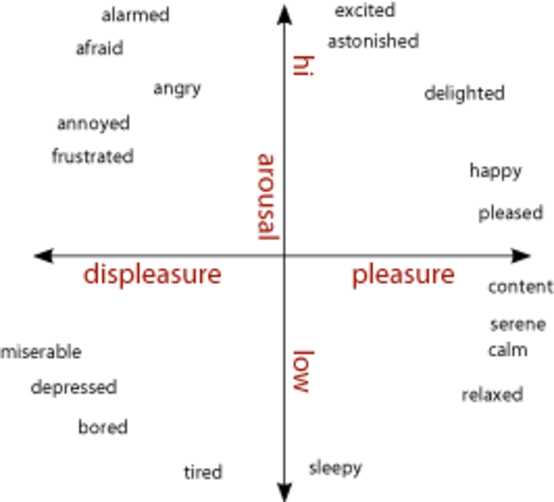
\includegraphics[width=0.5\textwidth]{images/russell-av-space.pdf}
  \label{fig:russelavspace}
\end{figure}

\footnotetext{Photo credit: http://imagine-it.org/gamessurvey/}

Both mentioned models for identifying emotions convey some
practical issues in emotion measurement. In a HCI context, the 
stimuli for potential emotions may vary less than
in human-human interaction (e.g., participant verbal expressions and body language) 
~\cite{zhang2010service} and also the combination of
evoked emotions ~\cite{peter2006emotion}. However with help of physiological
signals and the fuzzy logic in the model we are going to
use, such issues with our dimentional emotion models would
be minimized. Though it is anticipated to observe different range 
of evoked emotions while interacting with play
technologies compared to interacting with other humans in
daily life. ~\cite{zhang2010service}. However our dimensional emotion models
suffers some other problems. One problems is that arousal
and valence are not independent and one can impact the
other ~\cite{mandryk2007fuzzy}. Continuously capturing emotional experiences
in this applied setting is of its other hallmarks. Subjective
measures based on dimensional emotion theory, such as the
Affect Grid ~\cite{russell1989affect} and the Self-Assessment 
Manikin ~\cite{bradley1994measuring}, allow
for quick assessments of user emotional experiences but they
may aggregate responses over the course of many events ~\cite{zhang2010service}.
This work uses Mandryk et al. version of AV space ~\cite{mandryk2007fuzzy}.

%%%-----------------------------------------------------------------------------

\section{Measuring Affect}
%%% Talk about various sensors and their attributes, in particular the GSR sensor
%%% and how it can be used to detect Arousal using the fazzy logic

%%%-----------------------------------------------------------------------------

\section{Affect and Play Technologies}
%%% talk about play technologies and why do people play them
%%% the importance of being challenged in play technologies
%%% and its effect on arousal level

%%%-----------------------------------------------------------------------------

\section{Real Time Game Adaptation}
%%% talk about works has beed done in this area and different approaches
%%% and relate that to what we have done in this research

%%% adaptive play technologies critique existing systems (easy medium hard system), ideas
%%% , problems and challenges, works has been done, goals for this study and future works.
%%% adapting play technologies by chaning Player, NPC, Environment parameters.
%%% getting challenged and physiological signals, the importance of GSR

Playing video games as a kind of entertainment would help people to have new internal 
experiences. The virtual world of video games let adults to play as new rolls and enjoy filling 
their heads with new thoughts and emotions. Some people value 
the sensation

Games are opportunities for development and design of environments therefore 
the player can interactively experience various emotions and mental conditions.
This interactive experience in contrast to cinema 
and other major types of entertainment is what makes them exceptional

%%%-----------------------------------------------------------------------------

\chapter{Customizing Play Experience in Real-Time}    10 to 15 pages
- talk about various game design elements, player, npcs and environment 
and their connection to the play experience
- talk about the sensors and the fuzzy framework for emotion recognition
and connect that to the game design elements

\chapter{Implementation and Integration}              % 10 to 15 pages
% talk about various aspects of system's implementation and
% how it is integrated with the interactive technology
% - talk about the sensors and the fuzzy framework for emotion recognition
% and connect that to the game design elements

\section{Recognizing Emotion} %revision: 0
Heart rate (HR), blood pressure, respiration, electrodermal activity (EDA) and galvanic skin response (GSR), as well as facial EMG (Electromyography) are of physiological variables correlated with various emotions most. Interpreting physiological measures into emotion state can be difficult, due to noisy and inaccurate signals, however recent on-going studies in this area by Mandryk and Atkins ~\cite{mandryk2007fuzzy} presented a method to continuously identifying emotional states of the user while playing a computer game. Using the dimensional emotion model and the fuzzy logic, based on a set of physiological measures, in its first phase, their fuzzy model transforms GSR, HR, facial EMG (for frowning and smiling) into arousal and valence variables. In the second phase another fuzzy logic model is used to transform arousal and valence variables into five basic emotion states including: boredom, challenge, excitement, frustration and fun. Their study successfully revealed self-reported emotion states for fun, boredom and excitement are following the trends generated by their fuzzy transformation. The advantage of continuously and quantitatively assessing user's emotional state during an entire play by their fuzzy logic model is what makes their model perfect to be in incorporated with real-time play technologies. Therefore extracting user's emotional state as a new class of unconscious inputs to the play technology.


\section{Affect Engine} %revision: 2
Affect Engine is the software unit developed to transform collected physiological data to their equivalent emotional state in real-time. While it is generally agreed that emotions comprise three components: subjective experience (e.g. feeling joyous), expressive behavior (e.g. smiling), and physiological activation (e.g. arousal) ~\cite{scherer1993neuroscience}, Affect Engine provides a framework for transformation of physiological activations and some expressive behaviors. Affect Engine consists of four major components: Sensor Module, Fuzzification Module, Administration Panel and Engine Proxies, Figure \ref{fig:affect-engine} is a schematic view of these components working together. Applications such as games can easily integrate the Affect Engine where emotion recognition can offer adaptive control to maintain user interest and engagement. Once connected via sensors to the emotion recognition system, the affective state of the user can be captured continuously and in real-time, and used as a secondary input in the game logic for an enhanced play experienced.

\img
{Affect Engine}
{Affect Engine}
{placeholder.png}
{gsr-attached}

At the following a brief description on these components is provided.

\subsection{Sensor Module} %revision: 3
The sensor module consists of a Thought Technology ProComp Infinity encoder ~\cite{tt2013procomp} Figure ~\ref{fig:encoder}, connected to PC with a USB cable, SensorLib as the basic application programming interface (API) receives raw physiological inputs from the encoder driver and provides functionalities to apply different filters such as low-pass, high-pass, smoothing and shifting to the signal.

\img
{Thought Technology ProComp Infinity Encoder}
{Thought Technology ProComp Infinity Encoder}
{encoder.png}
{encoder}

\subsection{Fuzzification Module} \label{subsec:fuzzi} %revision: 3
This module functions through two separate phases; Then filtered signals are fuzzified using a set of fuzzy rules in the first phase of transformation. Then generated arousal and valence values are transformed into emotion values using another set of fuzzy rules in the second pass ~\cite{mandryk2007fuzzy}. A sample set for fuzzy rules used in the first and the second phase can be found in Appendix ~\ref{app:phys-to-av} and ~\ref{app:av-to-emotion}.



\subsection{Administration Panel}

\img
{Administration Panel}
{Administration Panel}
{placeholder.png}
{administration-panel}

\subsection{Engine Proxies}


\section{Sensors}
While the modular design of the Affect Engine allows its expansion for support of any physiological measures, currently the system uses Blood Volume Pulse (BVP), Galvanic Skin Response (GSR) and Electromyography (EMG; for frowning and smiling), to classify human affective states in 2-dimensional valence/arousal space (Figure \ref{fig:russelavspace}).

\subsection{Blood Volume Pulse and Heart Rate}
The Blood Volume Pulse (BVP, Figure \ref{fig:bvp-sensor}) is a relative measure of the amount of blood owing in a vessel. Using BVP we calculated heart rate and heart rate variability. The heart rate is known to reflect emotional activity and has been used to differentiate between both negative and positive emotions as well as different arousal levels ~\cite{tt2013procomp}.

\img
{Blood Volume Pulse (BVP) Sensor}
{Blood Volume Pulse (BVP) Sensor}
{bvp-sensor.png}
{bvp-sensor}

\subsection{Galvanic Skin Response}
The Galvanic Skin Response (GSR, Figure \ref{fig:gsr-sensor}) is useful to measure the skin's conductance between two electrodes and is a function of sweat gland activity and the skin's pore size. As a person becomes more or less stressed, the skin's conductance increases or decreases proportionally ~\cite{picard2003affective}.

\img
{Galvanic Skin Response (GSR) Sensor}
{Galvanic Skin Response (GSR) Sensor}
{gsr-sensor.png}
{gsr-sensor}

\subsection{Facial Electromyography}


\section{Integration with Valve Source Engine}
% talk about Modding Half Life EP2
\subsection{Level Design}
\subsection{The Director}

\chapter{Experimentation}                             % 5 to 10 pages
% talk about the experimentation
% adequacy, efficiency, productiveness, effectiveness
% (choose your criteria, state them clearly and justify them)
% be careful that you are using a fair measure, and that you are
% actually measuring what you claim to be measuring
% if comparing with previous techniques those techniques
% must be described in Chapter 2
% be honest in evaluation
% admit weaknesses

\section{Introduction}

\section{Experiment}


\section{Participants}
Data were recorded from 15 male and 1 female University students, aged between 18 and 32 (M = 25.00, SD = 3.875). As part of the experiment procedure demographic data were collected with special respect to the suggestions made by ~\cite{?}. Of the participants 94.1\% were right-handed. 41.2\% of participants rated their computer skills as Advanced while the rest of 58.8\% rated their skills as Intermediate. 35.3\% of participants have described themselves playing video games every day, while 41.2\% of them described themselves playing video games a few times per week and 17\% have been playing video games a few times per month and the rest of 5.9\% have been playing video games a few times per year. All participants have used PC as gaming system while 76.48\% of them also have used at least one of the four popular console platforms (XBox360, PS3, PS2, Wii) for gaming. All of participants had at least some experience with 3D shooting games like First Person Shooters. 47.1\% have described themselves playing 3D shooting games many times, while another 41.2\% described themselves as experts in 3D shooting games; Only a total of 11.8\% had limited or intermediate experience with 3D shooting games. Among the participants only 5.9\% had intermediate experience in using mouse in games, 35.3\% of them declared using mouse in games for many times and other 58.8\% of them described themselves as experts in doing that.

\section{Design}

A four condition (standard, player, NPC, environment) play session was employed to evaluate performance and excitement as dependent variables. The order 4 Latin square used to permute conditions between participants was as the following:

\centerline{a b c d}
\centerline{b c d a}
\centerline{c d a b}
\centerline{d a b c}

%%%%%%%%% nasty
at the start of the play session, they were required to press one of the four buttons on the entrance ramp labeled 1 to 4, and when any one of these buttons were pressed, the Affect engine started calibrating players signals for 60 seconds, during the calibration mode, no adjustment to any of game parameters is applied, no matter which condition is being played. After the one minute of calibration the system decides the standard range of signal for player's excitement value. After that except for the condition number 1 which is the no adaptation mode, the captured excitement value is normalized in the calibrated player range of excitement into a value between 0 and 1, and this value is then used to adjust the game parameters, this process of capturing, adjusting and applying the signal value would continue for 3 minutes until the next cycle of calibrating and adjustment starts. The player is required to play every condition for at least 5 minutes to ensure capturing of a complete cycle of calibrating and adjustment. After playing each condition, the player is asked to rest for 7 minutes, during this time the player is asked to fill out between condition questionnaires, which tries to ask the participant to self-estimate his affect level. The Player Mode is labeled as condition number 2, the NPC mode is labeled as condition number 3 and the Environment mode is labeled as condition number 4. From the 17 participants in this study, one has been lacking adequate level of expertise and therefore was unable to continue doing the required tasks at the expected level and therefore his results was not usable for this study. The image of signal values for this participant is depicted at the following:
%%%%%%%%% nasty

\section{Procedure}

The experiment was piloted with six participants (2 female). Pilot participants were selected from the Interaction Lab at the University of Saskatchewan, their comments on different mechanisms and online questionnaires of the experiment were reviewed to make participant more comfortable and less intervened during the experiment. Also pilot participants physiological data was recorded to confirm the functionality of the system during the experiment.

All experiments were conducted on weekdays, with the first slot beginning at 11:00h and the last ending at 18:30h. Participants were contacted to choose their preferred time slots while general time for one experimental session was 1:30 hours with setup and cleanup. Participants were invited to a laboratory, after a brief introduction of the experimental procedure, and becoming aware of the data being collected during the session, they were asked to fill out and sign informed consent form, this was the only paper form used during the experiment. Then the GSR sensors were attached to participant's hand.

Attached GSR sensors wired to the signal decoder brings limitations for participants while moving and using their hand. To diminish noisy signals and make participants feel comfortable under these limitations, the GSR sensors were attached to the hand that was handling the mouse during the game. While fingers dealing with mouse were quite steady compared to the other hand handling the keyboard, those fingers used to press the left and right mouse buttons were usually most comfortable ones for attaching GSR sensors. Some participants used index and middle fingers to press mouse buttons and others used index and ring fingers to do that \ref{fig:gsr-attached}.

\begin{figure}[h!]
  \caption[Attaching GSR sensors]
  {GSR sensors attached to index and middle finger of participant's right hand}
  \centering
  
\includegraphics[width=0.5\textwidth]{images/placeholder.png}
  \label{fig:gsr-attached}
\end{figure}

Having GSR sensors attached, participants were seated in a comfortable office chair, which was adjusted according to their individual height. They were then led to fill out the initial game demographic questionnaire. To keep GSR sensors attached during the experiment, all questionnaires after attaching GSR sensors were filled out using mouse and the same computer system. After the demographic questionnaire, participants were asked to self-assess their arousal, valence and dominance level using the self assessment manikin (SAM) questionnaire ~\cite{?}. Filling initial questionnaires after attaching GSR sensors was meant to give enough time (approximately 5 minutes) to the participant to get used to the sensors before playing the game. Participants then have been taken to a tour in the game. Different game mechanics were shown to them, and they were given about 1 minute, dependent to their experience, to make themselves comfortable with it. Some participants didn't need this time due to prior experience and asked to skip that. Then, participants played four different game conditions described before. Participants were not told about the differences between conditions. Each game condition was set to take 5 minutes. After each condition, participants were asked to write their comments about particular changes they noticed under that condition and its effect on their gameplay. Then they were asked to filled out the intrinsic motivation inventory (IMI) questionnaire, the player experience of need satisfaction (PENS) questionnaire and the game engagement questionnaire (GEQ) to rate their experience. Filling the questionnaires between conditions was done during the minimum 7 minutes of resting time before the next condition begins. The resting time was meant to restore players baseline signals. GSR sensors were recording players signals during both the play and the resting sessions from the beginning of the first condition to the ending of the last condition. After completion of the experiment, sensors were removed. Participants were debriefed and compensated \$15 Canadian dollars and escorted out of the lab.

\section{Materials and Measures}
\subsection{GSR}

\subsection{Subjective Measurements}

Participants were assessing their experience under different conditions, using four online questionnaires. FluidSurveys was used to host the questionnaires.

\paragraph{Self-Assessment Manikin}

After each condition participants were asked to rate the condition using 5-point Self-Assessment Manikin (SAM) \cite{bradley1994measuring} scale for arousal, valence and dominance. \textregistered FluidSurveys Multiple Choice widget was modified to include the SAM scales. Figure ~\ref{fig:sam} shows the arousal, valence and dominance scales used.

\begin{figure}[h!]
  \caption[Self-assessment manikin]
  {Self-assessment manikin for arousal, valence and dominance used after each condition and before the first condition}
  \centering
  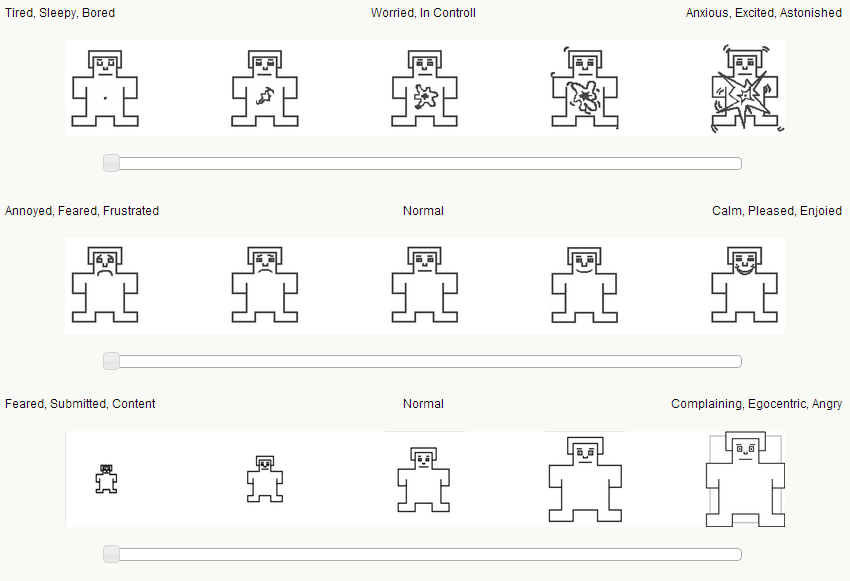
\includegraphics[width=0.7\textwidth]{images/sam.png}
  \label{fig:sam}
\end{figure}

\paragraph{Intrinsic Motivation Inventory}

Different components of game experience were measured using the Intrinsic Motivation Inventory questionnaire \cite{?}. It combines several game-related subjective measurement dimensions: interest/enjoyment, perceived competence, effort and felt pressure and tension while playing the game. Each one of these components consists of ?? question items (e.g., ``While playing, I was thinking about how much I enjoyed it'' is a interest/enjoyment component item). Question items were shown in a randomized order every time the page was viewed. Each question item consists of a statement on a five-point scale ranging from 1 (strongly disagreeing with the statement) to 5 (strongly agreeing with the statement). The questionnaire was developed based on survey studies \cite{?}.

\paragraph{Player Experience of Need Satisfaction}


\paragraph{Game Engagement Questionnaire}

%%%%%%%%%%%%%nasty%%%%%%%%%%%%%
An image of a regular participant signal values is depicted at
the following. In this image from left to right the light blue line
shows different conditions being played, and when the light blue
line is declining towards its base value, that is the period that
participant is asked to stop playing and instead relaxing and filling
out the questionnaires. The blue line is the normalized GSR signal
value of the participants which is used as an estimation of his
excitement level. The yellow green and pink lines are showing the
three different modes of Player, NPC and Environment parameters
being adapted

Following image is the GSR signal of players playing different
conditions from 1 to 4. From left to right the conditions are the
Default, Player, NPC and the Environment mode. This signals are all
based to an initial start value of 100, during the play experience,
some of them had gone bellow the start point and some other had risen
above that. Also the start time for each different condition is
shifted 500 seconds times the number of condition, from 0.

The following image is the average of GSR values for players in four
different conditions from left to right: Default, Player, NPC and
Environment modes
%%%%%%%%%%%%%nasty%%%%%%%%%%%%%

\section{Results}


% describe 16 participant's feedbacks and comments, and general ideas on how each one of them migh have experienced different situations through the game.


\chapter{Discussion}                                  5 to 10 pages
talk for the discussion
State what you've done and what you've found
Summarize contributions (achievements and impact)
Outline open issues/directions for future work

%-------------------------------------------------------------------------------

% Bibliography
\uofsbibliography[plain]{content/bibliography}

%-------------------------------------------------------------------------------

% APPENDICES
\uofsappendix
\chapter{Fuzzy Functions} put fuzzy functions here

%-------------------------------------------------------------------------------

\end{document}

%-------------------------------------------------------------------------------
